\documentclass[12pt]{article}
\usepackage[hcentering,bindingoffset=20mm]{geometry}
\usepackage{placeins}
%\usepackage[numbib]{tocbibind} use for ref in table of contents
\usepackage{rotating}
%\usepackage[natbibapa]{apacite}
%\usepackage[square,sort,comma,numbers]{natbib}
\usepackage{natbib}
\usepackage{graphicx}
\usepackage{tabularx}
\linespread{1.3}
\usepackage{gensymb}
\usepackage{longtable}
\usepackage{lscape}
\usepackage{url}
\addtolength{\textwidth}{2cm}
\addtolength{\hoffset}{-1cm}
\addtolength{\textheight}{2cm}
\addtolength{\voffset}{-1cm}
\setlength{\parindent}{0pt}
\title{Development of quantitative PCR assays for the detection and enumeration of toxic \emph{Gambierdiscus lapillus} and \emph{Gambierdiscus polynesiensis} (Gonyaulacales, Dinophyceae).}
\author{Key words:Ciguatera fish poisoning, \emph{Gambierdiscus lapillus},\\ \emph{Gambierdiscus polynesiensis},
 Quantitative PCR assay}
\date{}
\begin{document}
\maketitle
\paragraph{}A. L. Kretzschmar\\
Climate Change Cluster (C3), University of Technology Sydney, Ultimo, 2007 NSW, Australia, anna.kretzschmar@uts.edu.au
\paragraph{}A. Verma \\
Climate Change Cluster (C3), University of Technology Sydney, Ultimo, 2007 NSW, Australia
\paragraph{}G. S. Kohli\\
Climate Change Cluster (C3), University of Technology Sydney, Ultimo, 2007 NSW, Australia\\
Singapore Centre for Environmental Life Sciences Engineering (SCELSE), Nanyang Technological University, Singapore 637551, Singapore
\paragraph{}S. A. Murray\\
Climate Change Cluster (C3), University of Technology Sydney, Ultimo, 2007 NSW, Australia
\newpage
\section*{Abstract}
Ciguatera fish poisoning is an illness contracted through the ingestion of seafood containing ciguatoxins. 
It is prevalent in tropical regions worldwide, including in Australia. 
Ciguatoxins are produced by some species of \emph{Gambierdiscus}. 
Therefore rapid \emph{Gambierdiscus} species identification through quantitative PCR (qPCR), along with its toxicity, are required to screen for potential ciguatera risk development. 
In Australia, the identity, distribution and abundance of species of \textit{Gambierdiscus} that produce ciguatoxins is largely unknown. 
In this study we developed rapid qPCR assays to quantify the presence and abundance of two candidate species of \textit{Gambierdiscus} that may produce ciguatoxins in the region. %We determined the toxicity of the species \textit{G. lapillus} and \textit{G. polynesiensis}, and 
We assessed the specificity and efficiency of the  qPCR assays targeting \textit{G. lapillus} and \textit{G. polynesiensis}. 
The assays were tested on samples from 33 sites around Heron Island in the southern Great Barrier Reef semi-quantitatively, to determine the presence and patchiness of these species across samples from several macroalgal hosts.  


\newpage
\section*{Introduction}
%The genus Gambierdiscus and its morphological diversity, and why qPCR is needed to detect species.
Benthic dinoflagellates of the genus \emph{Gambierdiscus} Adachi \& Fukuyo produce ciguatoxins (CTX), which can accumulate in humans via consumption of contaminated seafood and cause ciguatera fish poisoning (CFP). 
Symptoms of CFP are largely gastrointestinal and neurotoxic however in severe cases humans can develop cardiovascular symptoms \citep{sims1987theoretical}. 
Species of \emph{Gambierdiscus} can be epiphytic, growing on macroalgae and other substrates such as dead coral, as well as traverse the water column. 
Species of \textit{Gambierdiscus} can vary in the production of ciguatoxins and/or maitotoxins \citep{chinain2010ciguatera,kohli2014high}. 
If a particular \emph{Gambierdiscus} sp. is a CTX producer, and inhabit a palatable macroalgal substrate, the toxins bioaccumulate in herbivorous fish and filter feeders with the potential to travel up the food chain to cause CFP in humans  \citep{chinain1997intraspecific,holmes1998gambierdiscus}. 

\emph{Gambierdiscus} was first identified in 1977, with the type species \emph{G. toxicus} Adachi \& Fukuyo \citep{adachi1979thecal}. 
The genus remained monotypic for 18 years until the discovery of a second species \emph{G. belizeanus} Faust \citep{faust1995observation}. 
To date, the genus comprises 14 described species and 6 ribo/species types
 \citep{smith2016new,fraga2016gambierdiscus,litaker2010global,adachi1979thecal,faust1995observation,chinain1999morphology,litaker2009taxonomy,dai2017taxonomic,nishimura2014morphology,rhodes2017new,kretzschmar2016characterization,fraga2011gambierdiscus,xu2014distribution,fraga2014genus} .
A major \emph{Gambierdiscus} species taxonomic revision was undertaken by Litaker et al. (2009). 
Reports of \emph{Gambierdiscus} spp. identified based on morphology alone, prior to this revision, need to be considered with caution as several new \emph{Gambierdiscus} spp. were defined. 
Further, intra-species variation and inter-species similarities can cause misidentification \citep{bravo2014cellular,kretzschmar2016characterization,kohli2014high}. 
Hence molecular genetic tools are important for determining the distribution and abundance of  \textit{Gambierdiscus} species and assess the risk of CFP in that region \citep{kohli2014high,kretzschmar2016characterization}. \\
%TODO Global Ecology and Oceanography of Harmful Algal Blooms ; chapter 13
%Toxins of Gambierdiscus. How to measure. Which species produce which toxins. Why this is important to know.
%check list of toxins 
\emph{Gambierdiscus} spp. produce a suite of different polyketide compounds - CTX, maitotoxin (MTX), gambierone, gambieric acid and gambierol have been characterised to date \citep{satake1993gambierol,nagai1992gambieric,rodriguez2015gambierone,murata1993structure,murata1989structures}. 
While any of these can contribute to toxicity, only CTX has been clearly linked to CFP in humans \citep{chinain1997intraspecific,holmes1998gambierdiscus}. 
The toxin profile of many \textit{Gambierdiscus} species is not well understood, and many different assays have been used to determine CTX toxicity \citep{globalcig}. 
Bioassays, such as mouse bioassays and neuroblastoma cell-line bioassays are good indicators of the toxicity of an organism, however species/strain specific toxin profiles needs to be elucidated with LC-MS/MS in order to characterise individual toxin congeners \citep{diogened2014chemistry}. 
The toxin profile of \textit{Gambierdiscus polynesiensis} Chinain \& Faust is the only of \emph{Gambierdiscus} spp.
%contention Gurjeet: wants it as 'one of' not 'only'
whose production of CTX congeners (P-CTX-3B, P-CTX-3C, P-CTX-4A, P-CTX-4B and M-seco-CTX-3C) has been verified by LC-MS/MS in isolates from French Polynesia and the Cook Islands, and is thought to be the principal cause of CFP in the Pacific region \citep{chinain2010growth,rhodes2014production}. 
However recently, a \emph{G. polynesiensis} strain isolated from the Kermandec Islands, Pacific Ocean, did not exhibit CTX toxicity detectable by LC-MS/MS  \citep{rhodes2017epiphytic}.
An uncharacterised peak in the CTX phase of several strains of \emph{Gambierdiscus lapillus} extracts was reported via LC-MS/MS, which did not match any available CTX standards (CTX-3B, CTX-3C, CTX-4A, CTX-4B) \citep{kretzschmar2016characterization}. 
Therefore, this species may produce previously uncharacterised CTX congener(s), and its production of CTX compounds requires further investigation.
Determining the toxin profile of \textit{Gambierdiscus} species requires toxin standards for comparative peak analysis. 
However, these are currently not commercially available. 
Therefore, progress in determining the toxins produced by species of \emph{Gambierdiscus} has been comparatively slow.\\

%CFP 
%CFP presents with over 175 gastrointestinal, cardiovascular and neurological symptoms and can be misdiagnosed \citep{sims1987theoretical,lindsay1997chronic,ting2001ciguatera,adams1993outbreak}. Dominant symptoms of CFP vary between geographic regions, which could be due to the different prevalent CTX congeners \citep{lewis2000ciguatera,dickey2010ciguatera}. The correct diagnosis relies on specific training of the physician which contributes to the low report rate globally.

CFP was given the "neglected tropical disease" status by a panel of experts co-ordinated by the Intergovernmental Oceanographic Commission’s (IOC) Intergovernmental Panel on Harmful Algal Blooms (IPHAB), as part of the United Nations Educational, Scientific and Cultural Organization), and a global ciguatera strategy was developed \citep{globalcig}. 
One element of the IOC/IPHAB ‘Global Ciguatera Strategy’ is to  investigate various species of the genus \emph{Gambierdiscus}, determine which species produce CTXs through LC-MS/MS and other means, and develop efficient and reliable molecular monitoring tools for the species of interest \citep{globalcig}. 
Quantitative PCR (qPCR) is a useful molecular genetic screening tool, as it can give species-specific and quantitative results from DNA samples extracted from environmental samples \citep{globalcig}. \\

%pPCR
qPCR is a variant of PCR in which a fluorescent agent is included in the PCR mix. 
Assays using qPCR have been extensively developed for the quantification of species of phytoplankton, particularly those involved in harmful algal blooms, utilizing methods such as SYBRgreen, Taqman assays, and others e.g. \citep{murray2011sxta,antonella2013quantitative,smith2009advantages,nishimura2016quantitative,vandersea2012development,hariganeya2013quantitative}. %Both these qPCR assay types have been successfully implemented in species specific environmental screening
\FloatBarrier
Currently there is one qPCR assay to identify the presence of the genera \emph{Gambierdiscus/Fukuyoa} \citep{smith2017molecular}. 
Assays for species specific identification are available for 6 of the 14 described \emph{Gambierdiscus} spp. and 3 out of 6 undescribed \emph{Gambierdiscus} sp. types/ribotypes (Table ~\ref{tbl:qpcrTable}). 
Assays are available for 2 of the 3 species of \emph{Fukuyoa} (Table ~\ref{tbl:qpcrTable}), which seceded from \emph{Gambierdiscus} as their own genus in 2015 \citep{gomez2015fukuyoa}. 
\textit{Fukoyoa} spp. are of interest for monitoring purposes as MTX producers, as the involvement of that toxin in CFP has not been resolved \citep{kohli2014feeding}.

%Which qPCR assays have been developed to date, why more are necessary

%Australia
In Australia, outbreaks of CFP occur annually in Queensland \citep{qldcig}. 
However, due to the complicated presentation of symptoms, the predicted report rate is less than 20\% \citep{lewis2006ciguatera}. 
Annually, there have been 7-69 reported cases between 2011 and 2015 (considering the report rate, $>$ 35-345 cases, see Table ~\ref{tbl:CFPTable}), with 2 fatalities reported in the state \citep{tonge1967ciguatera}. 
Cases of ciguatera from Spanish Mackerel fish caught in NSW have been reported since 2014 \cite{farrellclinical}, with five separate outbreaks affecting a total of 24 people since then \citep{farrell2017management}. 
Farrell et al. (2017) put forward a recommendation on how to manage the emerging ciguatera risk in NSW.
%Conversely, the fatal traffic accidents in Queensland in 2011 totalled 269 incidents \citep{qldtraffic}. Hence the potential number of ciguatera cases could exceed the fatal traffic accidents in Queensland in some years. 

Despite the prevalence of CFP in Australia, the characterization of \textit{Gambierdiscus} population is on going work. 
A causative species for CFP has not been identified and verified by LC-MS/MS to date, though recent work by Larsson et al. has identified several species that showerd ciguatoxin like activity in a bioassay \cite{larsson2018toxicology}.
%map of NSW outbreaks?
Over 50\% of Australia's expansive coastline (total 66,000 km) is tropical or subtropical, and may be considered potential habitat for \emph{Gambierdiscus} spp. \citep{kretzschmar2016characterization}. 
The 7 species of \emph{Gambierdiscus} that have been identified from Queensland and New South Wales are as follows: \emph{G. belizeanus} \citep{murray2014molecular}, \emph{G. carpenteri} \citep{kohli2014high,sparrow2017effects}, \emph{G. honu} (based on D8-D10 LSU sequence matching to a study by Richlen et al. \cite{richlen2008phylogeography}) \citep{rhodes2017new}, \emph{G. lapillus} \citep{kretzschmar2016characterization}, \emph{G. toxicus} \citep{hallegraeff2010algae} and two uncharacterized potentially new species \cite{larsson2018toxicology}, as well as \emph{F. yasumotoi}  \citep{murray2014molecular}). 
Using pyrosequencing, \textit{Gambierdiscus} was identified to the genus level in Western Australia \citep{kohli2014cob}, indicating that this is a coastline that should be examined further for CFP risk. 
qPCR primers that can be used for identification in Australia for potential monitoring purposes, have been developed for \emph{G. belizeanus}, \emph{G. carpenteri} and \emph{F. yasumotoi} \citep{nishimura2016quantitative,vandersea2012development}. 
Therefore, in order to assess the distribution and abundance of species that may produce CTXs in Australia, it is necessary to be able to assay the presence of other species in this region that are known to produce CTXs.\\ 


%aim
The aim of this study was to develop and test qPCR assays to detect the two species \emph{G. lapillus} and \emph{G. polynesiensis}. 
The latter is a species found in the Pacific that produces a range of CTXs congeners (CTX-3B, CTX-3C, CTX-4A, CTX-4B), identified by LC-MS/MS \citep{rhodes2014production}, and would be a plausible causative agent of CFP in Australia. 
The former is a recently identified species from the GBR with an unresolved toxin profile that indicates the possibility of CTX production.
\newpage
\section*{Materials and methods}
\subsection*{Clonal strains and culturing conditions}
Three strains of \emph{G. lapillus} and one strain of \emph{G.} cf. \emph{silvae} were isolated from Heron Island, Australia, as previously described \citep{kretzschmar2016characterization}. 
Two strains of \emph{G. polynesiensis} were isolated from Rarotonga, Cook Islands (table ~\ref{tbl:StrainTable}). 
The cultures were maintained F$\bullet$-10 medium at 27 $^{\circ}$C, 60mol$\bullet$-m$^{2}$ $\bullet$-s light in 12hr:12hr light to dark cycles.



\subsection*{DNA extraction and species specific primer design}
Genomic DNA was extracted using a modified CTAB method \citep{verma2016molecular}. 
The purity and concentration of the extract were measured using the Nanodrop (Nanodrop2000, Thermo Scientific), and the integrity of the DNA was visualised on 1\% agarose gel.
Unique primer sets were designed for the small-subunit (SSU) rDNA region of \emph{G. lapillus} and \emph{G. polynesiensis}, based on sequences available in the GenBank reference database. 
The target sequences were aligned against sequences of all other \emph{Gambierdiscus} spp. that were available on GenBank reference database, with the MUSCLE algorithm (maximum of 8 iterations) \citep{edgar2004muscle} used through the Geneious software, version 8.1.7 \citep{kearse2012geneious}. 
Unique sites were determined manually (Table ~\ref{tbl:PrimerTable}). 
Primers were synthesised by Integrated DNA Technologies (IA, USA).
Primer sets were tested systematically for secondary product formation for all 3 strains of \emph{G. lapillus} and 2 strains of \emph{G. polynesiensis} (Table ~\ref{tbl:StrainTable}) via standard PCR in 25$\mu$l mixture in PCR tubes. 
The mixture contained 0.6 $\mu$M forward and reverse primer, 0.4 $\mu$M BSA, 2 - 20 ng DNA, 12.5 $\mu$l 2xEconoTaq (Lucigen) and 7.5 $\mu$l PCR grade water.
The PCR cycling comprised of an initial 10 min step at 94 $^{\circ}$C, followed by 30 cycles of denaturing at 94 $^{\circ}$C for 30 sec, annealing at 60 $^{\circ}$C for 30 sec and extension at 72 $^{\circ}$C for 1 min, finalised with 3 minutes of extension at 72 $^{\circ}$C. 
Products were visualised on a 1\% agarose gel.


\subsection*{Evaluation of primer specificity}
To verify primer set specificity as listed in Table ~\ref{tbl:PrimerTable}, DNA was extracted via CTAB from \emph{G. australes} (CCMP1650 and CG61), \emph{G. belizeanus} (CCMP401), \emph{G. carpenteri} (UTSMER9A3), \emph{G. pacificus} (CAWD149) and \emph{G.} cf. \emph{silvae} (HG5). 
\emph{G. cheloniae} (CAWD232) DNA was extracted using a PowerSoil™ DNA isolation kit (Mo Bio Inc., CA, USA). 
\emph{G. scabrosus} (KW070922\_1) DNA was extracted using DNeasy Plant Mini Kit (Quiagen, Tokyo, Japan) according to the manufacturer's protocol. 
For all extracted samples, the presence and integrity of genomic DNA was assessed on 1\% agarose gel. 
Primer sets designed for \emph{G. lapillus} and \emph{G. polynesiensis} were tested for cross-reactivity against all other \emph{Gambierdiscus} spp. available via PCR (BioRadT100 Thermal Cycler (CA, USA)), appropriate positive and negative controls were applied. 
PCR amplicons were visually assessed on 1\% agarose gel.


\subsection*{Evaluation of primer sensitivity}
The qPCR reaction mixture contained 10 $\mu$l SYBR Select Master Mix (Thermo Fisher Scientific), 7 $\mu$l MilliQ water, 0.5 $\mu$M forward and reverse primers and 2 - 20 ng DNA template, for a final volume of 20 $\mu$l. 
Cycling conditions consisted of 10 min at 95, then 40 cycles of 95 $^{\circ}$C for 15 seconds and 60 $^{\circ}$C for 30 seconds, followed by a temperature gradient for melt curve construction.
\subsection*{Calibration curve construction}
Standard curves were constructed to determine the efficiency of the assay, using a synthetic gene fragment approach, and also to use to quantify species presence, using calibration curves based on DNA extracted from known cell numbers. 
For curves based on synthetic gene fragments, a 10-fold serial dilution of a synthesised fragment containing the SSU target sequence, forward and reverse primer sites and 50bp flanking both primer sites matching sequencing results was generated. Cell-based standard curves were constructed using 10-fold dilutions of gDNA extract of known cell concentrations.
The calibration curves for both methods were calculated (R$^{2}$, PCR efficiency and regression line slope) and graphed in R version 3.2.3 \citep{rlang}, using R studio version 1.0.136 \citep{rstudio} and the ggplot2 package \citep{ggplot2}. 
%AE is (10^(1/slope)-1)*100
\subsubsection*{Gene based calibration curve}
For the target amplicons of both \emph{G. lapillus} and \emph{G. polynesiensis}, a DNA fragment spanning the target sequence, the reverse and forward primer sites and an extra 50bp on either end was synthesised called gBlocks \textsuperscript{\textregistered} by Integrated DNA Technologies (IDT, IA, USA). 
Lyophilized gBlocks \textsuperscript{\textregistered} was re-suspended in 1x TE (Tris 1M, EDTA 0.5 pH8) to a concentration of 1 ng.$\mu$l. 
The copy number of gene fragment was then calculated as 28,850,000,000 and 24,380,000,000 for the \textit{G. lapillus} and \textit{G. polynesiensis} target rDNA regions respectively.
%inseet calculation
The stock solution was 10-fold serially diluted and dilutions between 10$^{3}$ and 10$^{8}$ were amplified by qPCR (on StepOnePlus System by Applied Biosystems (Thermo Fisher Scientific, Waltham, MA, USA) and BioRad (CA, USA) CFX96 real time systems for \emph{G. lapillus} and \emph{G. polynesiensis} respectively) in triplicate.


%add more info
\subsubsection*{Cell based calibration curve}
Two strains of \emph{G. lapillus} (HG4 and HG7) and \emph{G. polynesiensis} (CG15) (Table ~\ref{tbl:StrainTable}) were used to construct cell based standard curves. 
Cells were counted using a Sedgwick Rafter counting chamber as viewed under a Nikon Eclipse TS100 (Australia) microscope. 
DNA was extracted with the FastDNA spin kit for soil by MP Biomedicals (CA, USA), as per the manufacturer's instructions. 
The gDNA extracts were 10-fold serially diluted. 
Dilutions ranging from 3880 to 0.0388 cells, 5328 to 0.05328 and 4035 to 0.4035 for HG4, HG7 and CG15 respectively. 
Samples were amplified via qPCR (on StepOnePlus System by Applied Biosystems (Thermo Fisher Scientific, Waltham, MA, USA) and BioRad (CA, USA) CFX96 real time systems for \emph{G. lapillus} and \emph{G. polynesiensis} respectively) in triplicate.

\subsection*{Determination of extractable gene copies per cell for \emph{G. lapullis} and \emph{G. polynesiensis}}

To determine the extractable mean SSU rDNA copies per cell, the known cell counts for the cell based calibration curve were used as input for calculation. 
Copy number was defined as a linear regression of the gene based calibration curve using the input cell counts to determine extractable SSU rDNA copy number per cell.

\subsection*{Screening environmental samples for \emph{G. lapillus} and \emph{G. polynesiensis} abundance}
Around Heron Island and Heron Reef (Fig. ~\ref{fig:samplesites}) 33 sites (within 1km of the shore) were sampled in October 2015, in spatial replicates (A, B, C; Supplementary Table 1) within a 2m radius. 
Three species of macroalgae that commonly grow on this reef, \textit{Chnoospora} sp., \textit{Padina} sp. and \textit{Saragassum} sp., were sampled for the presence of epiphytic \emph{Gambierdiscus} spp. For each sample, about 200 g of macroalgae was collected from approximately 1 m deep water at low tide and briefly placed in plastic bags containing 200 to 300 ml of ambient seawater. 
They were shaken vigorously for 5 min to detach the epiphytic dinoflagellates from the macroalgae. 
This seawater was passed through $>$ 120 μm mesh filter to remove any remaining larger fauna and debris. 
The collected seawater was centrifuged at 1000 rpm. The supernatant was discarded and the pellet was dissolved in 10 ml RNAlater (Ambion®, Austin, TX, USA) for preservation and stored at 4$^{\circ}$C.
To assess the presence of these species in the pelagic environment adjacent to macroalgal beds, plankton nets were dragged through the current (samples 34 - 38; Supplementary table 2) for five minutes, then processed as macroalgal samples.
Samples were screened in triplicate for both \emph{G. lapillus} and \emph{G. polynesiensis} on a StepOnePlus System by Applied Biosystems (Thermo Fisher Scientific, Waltham, MA, USA).



\newpage
\section*{Results}
\subsection*{Evaluation of primer specificity}
The qGlapSSU2F - qGlapSSU2R primer pair (Table ~\ref{tbl:PrimerTable}) amplified in PCRs of all five strains of \emph{G. lapillus}, while no amplification was observed for genetically closely related species \emph{G. belizeanus}, \emph{G. cheloniae}, \emph{G. pacificus} and \emph{G. scabrosus}. 
Other species of \emph{Gambierdiscus} from different clades, \emph{G. australes}, \emph{G. carpenteri}, \emph{G. polynesiensis} and \emph{G.} cf. \emph{silvae} (Table ~\ref{tbl:CrossreactTable}) were not amplified using these primer pairs \citep{smith2016new,kretzschmar2016characterization}.

In PCRs using the qGpolySSU2F - qGpolySSU2R primer set, \emph{G. polynesiensis} amplified while species from the same genetic clade, \emph{G. australes} and \emph{G.} cf. \emph{silvae}, did not amplify. 
No amplification was observed for \emph{Gambierdiscus} species tested from different clades: \emph{G. belizeanus}, \emph{G. cheloniae}, \emph{G. lapillus }\emph{G. pacificus} and \emph{G. scabrosus} (table ~\ref{tbl:CrossreactTable}) \citep{kretzschmar2016characterization}.


 
\subsection*{Evaluation of primer sensitivity}
The cell-based standard curves for \emph{G. lapillus} (HG4 and HG7, Fig. ~\ref{fig:stdCurve}a) showed high linearity with R$^{2}$ approaching 1.00. 
The slope for the Ct vs. log$_{10}$ cell number for HG4  was -3.4, efficiency 96.8 \%%  and amplification factor 1.97
; and -3.51, efficiency of 92.7 \% %  with an amplification factor of 1.93
for HG7. The linear detection for both \emph{G. lapillus} isolates covered six orders of magnitude. 
The lowest number of cells detected were 0.04 and 0.05 cells for HG4 and HG7 respectively (Fig. ~\ref{fig:stdCurve}a).
The detection for \emph{G. polynesiensis} CG15 was over five orders of magnitude with a lowest detection was of 0.4 cells (Fig. ~\ref{fig:stdCurve}b) and showed high linearity with R$^{2}$ equals 1.00. 
The slope for the Ct vs. log$_{10}$ cell number was -4.35 with a PCR efficiency of 70 \%.



The gene based standard curve for \emph{G. lapillus} covered linear detection over 7 orders of magnitude, with a slope of -3.42, R$^{2}$ equals 0.99 and a PCR efficiency of 96 \%. %The detection limit tested was less than 10$^{5}$ gene copy numbers. The Ct for the lowest gene copy number tested was less than 25, so it is likely that the sensitivity is lower than 10$^{5}$ gene copy numbers.\\
The \emph{G. polynesiensis} gene based standard curve covered six orders of magnitude, with a slope of -4.15, R$^{2}$ equals 1.00 and a PCR efficiency of 74.2 \%.



%Ct of known gBlocks gives copy number - extrapolate those to SSU rDNA copies for cell. can compare to
\subsection*{Quantification of extractable SSU rDNA copy number per cell of \emph{G. lapillus} and \emph{G. polynesiensis}}
The detectable SSU copies for \emph{G.lapillus} were 22,430 and 5,855 copies per cell for HG4 and HG7 respectively. For \emph{G. polynesiensis} (CG15) the detectable copy number of SSU was 4,924 copies per cell.

\subsection*{Screening environmental samples for \emph{G. lapillus} and \emph{G. polynesiensis} abundance}
To evaluate the adequacy of the \emph{G. lapillus} and \emph{G. polynesiensis} qPCR assays for environmental screening, the assays were applied to environmental community DNA extracts collected around Heron Island. 
Low cell numbers were detectable for \emph{G. lapillus}. 
\emph{G. polynesiensis} was not detected in any of the environmental samples (Supplementary Table 1).
Ct values for \emph{G. lapillus} detection in environmental samples were calibrated to the HG7 standard curve and calculated as cells per gram wet weight macroalgae (Supplementary Table 1). 
\emph{G. lapillus} was detected across 32 of the 33 sampling sites. Sites at which \textit{G. lapillus} was present, it showed a patchy distribution, being present at two of the three spatial replicates in the majority of samples (23 of 33 sample sites), followed by all three spatial replicates testing positive (8 out of 33 sites) and at one site only one of the spatial replicates was positive (Fig. ~\ref{fig:envposneg}). \\
\emph{G. lapillus} was detected at 71 out of the 99 spatial replicates, specifically at 23/30, 18/28 and 9/10 samples from \emph{Chnoospora} sp., \emph{Padina} sp. and \emph{Saragassum} sp. as substrate respectively, as well as 26/31 sites sampled from mixed macroalgae (Supplementary Table 1).
Patchiness was also found in the abundance as wellas the distribution of \emph{G. lapillus}, from 0.24 cells.g$^{-1}$ wet weight macroalgae to 49.51 cells.g$^{-1}$ wet weight macroalgae, with a mean of 5.84 cells.g$^{-1}$ wet weight macroalgae. 
For example (6A - \emph{Chnoospora} sp.) and (6B - \emph{Padina} sp.) hosted comparable cell numbers (1.12 cells and 1.65 cells per g.ww algae respectively) while no \emph{G. lapillus} cells were detected on (6C - \emph{Padina} sp.).
Only at one of 33 sampling sites, no \emph{G. lapillus} presence was detected across all three spatial replicates (25A, B, C).
At all other sites, the presence of \textit{G. lapillus} varied between spatial replicates of but did not significantly differ between macroalgal host or location (Fig. ~\ref{fig:envHG7}). 

\newpage
\section*{Discussion}
%aim of study, ways to achieve aim, results, extrapolate for accurate tool development
The aim of the study was to design and validate qPCR assays to quantify the species \emph{G. lapillus} and \emph{G. polynesiensis}, which may produce CTX toxins in the Australian GBR region. 
Species-specific PCR primers with high specificity and sensitivity were developed and the SSU copy number for two strains per species were determined. 
We also established that these primer sets were effective in measuring the abundance and distribution of two \emph{Gambierdiscus} species at Heron Island reef. 
The cross-reactivity of primers designed in this study showed high specificity for both \emph{G. lapillus} and \emph{G. polynesiensis} individually while not amplifying when tested against other \emph{Gambierdiscus} spp. 
The species tested for cross-reactivity were chosen because they represented species that are most genetically similar to each target species for the SSU region (as per Fig. 2 in \citep{kretzschmar2016characterization}).
%insert the species tested and why
Standard curves were constructed for two strains of \emph{G. lapillus} and one strain of \emph{G. polynesiensis}, for which the primers showed high linearity and amplification efficiency (Fig. ~\ref{fig:stdCurve}). 
Hence these primer sets are accurate and reproducible molecular tools to enumerate the target species exclusively from environmental community DNA extracts.
Due to the potential CTX production of \emph{G. lapillus} \citep{kretzschmar2016characterization,larsson2018toxicology} and the established suite of CTX production of \emph{G. polynesiensis} from the South Pacific \citep{chinain2010growth}, their presence and distribution is of interest in Australia where the causative organism(s) for CFP is yet to be established.\\

%insert N2A info if available. Chinain 2010 shows a number of references that are related to strain variation in toxin production\\

%precise determination ofSSU important
As ciguatera risk is linked to the abundance of \emph{Gambierdiscus} species producing CTXs, it was important to establish a quantitative assay for detection.
For both species we validated synthetic gene fragment standard curves of the target region (gBlocks \textsuperscript{\textregistered}) and compared these to cell standard curves to establish 'absolute' qPCR assays \citep{nishimura2016quantitative,hariganeya2013quantitative}. 
Further, we determined the extractable copy SSU rDNA number for two strains of \emph{G. lapillus} (HG4 and HG7) and one strain of \emph{G. polynesiensis} (CG15). 
The copy number for both \emph{G. lapillus} (5855.3 to 22,430.3 rDNA copies per cell) and \emph{G. polynesiensis} (4,924 rDNA copies per cell) were comparable to the copy numbers determined by Vandersea et al. (2012), which ranged from 690 rDNA copies for \emph{G. belizeanus} to 21,498 copies for \emph{G. caribaeus}. 
In comparison the cell copy numbers determined by Nishimura et al. (2016) ranged from 532,000 copies for \emph{G. scabrosus} and 2,261,000 for \emph{G.} sp. type 3. While the difference in rDNA copy numbers may be due to inter-species differences, or even intra-species as per the \emph{G. lapillus} results, Nishimura et al. argue that the difference could be underestimation of rDNA copy numbers due to 'ghost' cells counted for total cell number which do not contribute to amplification \citep{nishimura2016quantitative,hariganeya2013quantitative}.
The difference in extractable SSU rDNA copies between the two strains of \emph{G. lapillus} is intriguing. 
As the variation between the two strains tested is within the observed variation reported by Nishimura et al. (2016) from single cell qPCR experiments for rDNA copy number elucidation, the difference reported here is likely representative of biological intra-strain variation rather than methodological artifacts. 
A 5-fold difference in toxicity between the same HG4 and HG7 strains for \emph{G. lapillus} was also reported by Kretzschmar et al. (2017), and there was a noticeable difference in growth rate between the two strains observed (but not quantified) in this study. 
The amounting evidence of intra-strain variability in toxicity, detectable rDNA copy numbers and potentially growth rate could have severe implications for qPCR based cell enumeration of environmental samples when attempting to extrapolate ciguatera risk and requires further investigation.\\
%TODO ^ negligeable dif in SSU# for cultured and wild type for 4 phylotypes therefore culture based std is adequate predictor for environmental cell numbers ~  detection limits --> Further, examining the difference in SSU copy numbers between 
The qPCR assays were successfully tested on environmental DNA extracts from around Heron Island, and gave some insight into \emph{G. lapillus} distribution and abundance. 
While \emph{G. polynesiensis} was not detected in any of the environmental samples, the qPCR primer set described here is sensitive and specific (Fig. ~\ref{fig:stdCurve}B, Fig. ~\ref{fig:lapigblocks}B), hence can be utilized for monitoring programs.
The qPCR assays detected \emph{G. lapillus} at all but one of the sites tested (Fig. ~\ref{fig:envposneg}). 
Within the spatial replicates, the distribution of \emph{G. lapillus} was patchy, as 25 of the 32 sites included one sample with no \textit{G. lapillus} present (Fig. ~\ref{fig:envposneg}). 
Patchiness in the distribution of \textit{Gambierdiscus} species has previously been found in a study of 7 \emph{Bryothamnion} macroalgae spaced 5 to 10 cm apart, in which 5 to 70 cells g-1 algae were found \citep{taylor1986underwater}.\\
%do damn stats
There was no significant difference in the presence/absence of \emph{G. lapillus} cells observed as per the macroalgal host, \emph{Padina} sp., \emph{Sargassum} sp. or \emph{Chnoospora sp.}.  \\
%nets
\emph{G. lapillus} was also detected in two of samples taken using a plankton net tow (Supplementary table 2). 
Motile behaviour has been observed previously in the field at various time points \citep{yasumoto1977finding,bomber1987ecology}. 
Parsons et al. (2011) reported \emph{Gambierdiscus} sp. behaviour as facultative epiphytes during lab scale experiments, as cells showed attachment as well as motile stages over time in the presence of different macroalgae \citep{parsons2011examination}. 
Taylor \& Gustavson (1983) reported that \emph{Gambierdiscus} cells were captured in plankton tows by de Silva in 1956 but reported as \emph{Goniodoma} \citep{taylor1986underwater}.

Across spatial replicates where \emph{G. lapillus} was detected, cell densities were consistent (Fig. ~\ref{fig:envHG7}). 
The average cell density of \emph{G. lapillus} 5.84 cells$^{-1}$g wet weight macroalgae, which is comparable to the cell densities recorded by Nishimura et al. (2016) in their environmental screening (Table 4 in \citep{nishimura2016quantitative}).\\
%insert other studiesof macroalgae colonization

 %For assessment of CFP risk, factors other than just \emph{Gambierdiscus} cell numbers are other factors at play. The toxicity of the species is essential in determining risk, and this could be subject to intra-strain variation \citep{kretzschmar2016characterization}. Furthermore, the type of macroalgal substrate is key. Cruz-Rivera et al. (2006) report several of the commonly habitated macroalgae are not palatable for herbivores, which suggests that the protist communities residing on their surface would not enter the food chain. They suggest that chemically and structurally defended macroalge could serve as a refugium for toxic \emph{Gambierdiscus} spp. Conversely, fast growing palatable hosts would serve as a consistent delivery mechanism of toxic \emph{Gambierdiscus} spp. for bioaccumulation. Low cell numbers in this scenario could still serve as the basis for a highly ciguateric trophic system, depending on the speed of uptake \citep{cruz2006macroalgal}.
%The brown macroalgae collected for this study vary in palatability and defence mechanisms(Appendix A in \citep{cruz2006macroalgal} and references therein): The palatability of \emph{Chnoospora} spp. is undocumented though quick response to nutrient pulses suggests fast growth rate; \emph{Padina} spp. vary in palatability depending on species in question and the herbivore; and \emph{Sargassum} spp. show high intra-species variability in palatability. \emph{G. lapillus} has also been isolated from  \emph{Halimeda}, a green algae with extensive chemical and structural defences which is rarely consumed by herbivores \citep{kretzschmar2016characterization,cruz2006macroalgal}.

%semi quant nature of screening
As many authors have pointed out (e.g. \citep{litaker2010global,bomber1989epiphytism,tester2014sampling,cruz2006macroalgal,parsons2011examination,globalcig,lobel1988assessment}), there are several difficulties in determining precise quantification of \textit{Gambierdiscus} species on macroalgae in order to assess potential ciguatera risk. 
Due to the difference in habitable surface area between samples taken from the structurally diverse macroalgae, including those sampled in this study (\emph{Chnoospora} sp., \emph{Padina} sp. and \emph{Sargassum} sp.), the potential habitable space is difficult to compare. 
In order to assess ciguatera risk in a given area, the properties of the macroalgae with \emph{Gambierdiscus} epiphytes need to be considered. 
If the macroalgae is structurally or chemically defended against herbivory, any CTX produced by the epiphytes is unlikely to enter the food chain \citep{cruz2006macroalgal}. 
Due to the difficulty in quantifying \emph{Gambierdiscus} on a particular substrate, Tester et al. (2014) proposed have the use of an artificial substrate (commonly available black fibreglass screen of a known surface area) and a standardised sampling method \citep{tester2014sampling}.




%discuss macroalgal sunstrate thing
%\emph{Gambierdiscus} spp. preferentially colonize some macroalgae over others. The preferences recorded in the literature are contradictory and indicate a \emph{Gambierdiscus} species specific perference (for a review see Parsons et al. (2011)).
%need to discuss literature entries
%Parsons et al. (2011) tested the the affinity and survivability of \emph{Gambierdiscus} clone BIG-12 in for 24 macroalgal specimens \citep{parsons2011examination}. The macroalgal hosts assessed were monitored on the basis of BIG-12 cell attachment, motile cells and cell death over time. They found that attachment and survival of \emph{Gambierdiscus} cells was limited for macroalgae that employ chemical defences against herbivory. This suggests that the macroalgae chosen for CFP screening should be considered for their attributes as a host and likely a range of samples should be screened.

%The study conducted by Pasons et al. (2011) using BIG-12 is the most extensive to date in terms of macroalgal preference and associated mortality. As preference differs between \emph{Gambierdiscus} species, the species designation is important. BIG-12 was identified as \emph{G. toxicus} using  the dichotomous species identification key proposed by Litaker et al. (2009) \citep{litaker2009taxonomy}. Kohli et al. (2014) morphologically identified \emph{Gambierdiscus} from Merimbula, Australia, as \emph{G. toxicus} however rTEFP analysis showed that it was \emph{G. carpenteri}. Further, morphological intra-species variation has been demosntrated in \emph{Gambierdiscus} spp.  \citep{bravo2014cellular,kretzschmar2016characterization,fraga2016gambierdiscus}.
%Hence the BIG-12 strain needs to be identified based on LSU or SSU rDNA for informative species specific colonization preference. 

%Here here we have demonstrated that \emph{G. lapillus} colonised \emph{Chnoospora} sp., \emph{Padina} sp. and \emph{Sargassum} sp. Further, \emph{G. lapillus} also colonised \emph{Halimeda} sp. \citep{kretzschmar2016characterization}.

% Look at actual cell numbers incl Nishimura cell numbers comparable table 4

%nishimura 16 no diff beteen cell growth phases and SSU # copy 
%The difference in SSU copy number between strains in both \emph{G. lapillus} (HG4 , HG7) and \emph{G. polynesiensis} (CG14 , CG15) could be due to a number of procedural problems: over or under estimation from cell counts due to non-uniform cell suspension of \emph{Gambierdiscus}; loss of cells during the standard curve DNA extraction; or change of in Ct values between runs. Precautions were taken to address these possibilities. The aggregation of \emph{Gambierdiscus} spp. has been reported by *CITE*. Hence cultures were heavily agitated before sample collection for counting. To account for DNA loss during extraction, the gBlocks standards were extracted by the same procedure as the cell based standards, modelled on the experimental procedure by Kon et al. (2015) \citep{kon2015spatial}. To avoid error from run based differences in Ct values, the same machine was used for all runs and sub samples of the cell standards included in the gBlocks run (as well as the environmental screening) to assess the experimental Ct value compared to a known Ct value. 
%Nishimura et al. (2016) assessed the SSU copy variation of \emph{G. scabrosus} at different growth phases and found no significant differences. 
%This indicates that the strain variation of \emph{G. lapillus} and \emph{G. polynesiensis} SSU copy numbers is likely not due to difference in growth phase when harvesting respective strains. 
%However this assumption should be taken with caution due to the findings in the closly related genus \emph{Alexandrium}, where \emph{Alexandrium catenella} displayed no growth phase dependent SSU copy variation while \emph{Alexandrium taylori} did \citep{galluzzi2010analysis}. %SM--> minor point

%SM --> minor point: Due to the synchronised growth and harvesting cycles, the intra strain variation in SSU copies in \emph{G. lapillius} is not dependent on growth phase variation. Subsequently, the estimation of cells in environmental samples by comparison to a cell based standard will likely be slightly inaccurate. However the discrepancy would be minor, so qPCR enumeration is still considered accurate and an adequate screening tool for monitoring. 

\section*{Conclusion}
The qPCR assays developed in this study are expedient and accurate molecular tools to detect and enumerate the present of \emph{G. lapillus} and \emph{G. polynesiensis} in environmental samples. 
The assays were shown to be highly sensitive and accurately detected cell 0.05 to over 4000 cells for \emph{G. lapillus} and 0.4 to over 4000 cells for \emph{G. polynesiensis}.
While \emph{G. polynesiensis} was not detected around Heron Island, this species is a LC-MS/MS verified CTX producer and therefore rapid environmental screening for this species is essential for ciguatera monitoring and in line with the Global Ciguatera Strategy. 
\emph{G. lapillus} may produce CTXs, but regardless is a part of the ciguateric web in Australia and was detected at most sites sampled.
The assays were applied to spatial replicates from 33 sites around Heron Island on the GBR, which found that proximity is a poor predictor of \textit{Gambierdiscus} presence.
%re-state aim w/ sensitivity etc, tool fort env monitoring, detection limits
%With the description of these primer sets, four of the five Australian \emph{Gambierdiscus} spp. can be monitored, sans \emph{G. toxicus}

\FloatBarrier
\begin{table}
\caption{Published qPCR assays for \emph{Gambierdiscus} and \emph{Fukoyoa} spp.}
\label{tbl:qpcrTable}
\begin{tabular}{ | p{6cm} | p{3cm} | p{3cm} | }
\hline
\textbf{Species} & \textbf{Method}& \textbf{Reference} \\
\hline
\multicolumn{3}{| c |}{\textbf{\textit{Gambierdiscus} spp.}}\\
\hline
\emph{G. australes}&TaqMan Probes&\citep{nishimura2016quantitative}\\
\hline
\textit{G. belizeanus}&SYBR Green&\citep{vandersea2012development}\\
\hline
\textit{G. caribaeus}&SYBR Green&\citep{vandersea2012development}\\
\hline
\emph{G. carolinianus}&SYBR Green&\citep{vandersea2012development}\\
\hline
\textit{G. carpenteri}&SYBR Green&\citep{vandersea2012development}\\
\hline
\emph{G. scabrosus}&TaqMan Probes&\citep{nishimura2016quantitative}\\
\hline
\textit{Gambierdiscus} sp. ribotype 2&SYBR Green&\citep{vandersea2012development}\\
\hline
\textit{Gambierdiscus} sp. type 2&TaqMan Probes&\citep{nishimura2016quantitative}\\
\hline
\textit{Gambierdiscus} sp. type 3&TaqMan Probes&\citep{nishimura2016quantitative}\\
\hline
\multicolumn{3}{| c |}{\textbf{\textit{Fukuyoa} spp.}}\\
\hline
\textit{Fukoyoa ruetzleri}&SYBR Green&\citep{vandersea2012development}\\
\hline
\textit{Fukoyoa} cf. \textit{yasumotoi}&TaqMan Probes&\citep{nishimura2016quantitative}\\
\hline
\end{tabular}
\end{table}
\FloatBarrier
\begin{table}
\caption{Cases of Ciguatera Fish Poisoning reported to health authorities in Queensland, Australia, between 2011 and 2015, by Queensland Health \citep{qldcig}.}
\label{tbl:CFPTable}
\begin{tabular}{ | p{6cm} | p{1.5cm} | p{1.5cm}| p{1.5cm} | p{1.5cm} | p{1.5cm} | }
\hline
Year &2011&2012&2013&2014&2015\\
\hline
Recorded CFP cases&18&7&25&69&11\\
\hline
Extrapolated CFP indcidences&$\sim$90&$\sim$35&$\sim$125&$\sim$345&$\sim$55\\
\hline
\end{tabular}
\end{table}
\FloatBarrier
\begin{table}
\caption{List of \emph{Gambierdiscus} clonal strains used for the qPCR assay.}
\label{tbl:StrainTable}
\begin{tabular}{ | p{2cm} | p{2cm} | p{2cm}| p{3cm} | p{3cm} | p{2cm} | }
\hline
\textbf{Species} & \textbf{Collection site} & \textbf{Collection date} &\textbf{Latitude} & \textbf{Longitude} & \textbf{Strain name} \\
\hline
\emph{G. lapillus} &Heron Island, Australia &July 2014 &23$^{\circ}$ 4420' S&151$^{\circ}$ 9140' E & HG4 \\
\hline
&&&&& HG6\\
\hline
&&&& &HG7\\
\hline
%&&&& &HG26\\
%\hline
\emph{G. polynesiensis}&Rarotonga, Cook Islands&November 2014 &21$^{\circ}$ 2486' S&159$^{\circ}$ 7286' W & CG14 \\
\hline
&&&&&CG15\\
\hline
\emph{G.} cf. \emph{silvae}&Heron Island, Australia &July 2014 &23$^{\circ}$ 4420' S&151$^{\circ}$ 9140' E& HG5\\
\hline
\end{tabular}
\end{table}
\FloatBarrier
\begin{table}
\caption{List of species specific qPCR primer sets for SSU rDNA.}
\label{tbl:PrimerTable}
\begin{tabular}{ | p{2.5cm} | p{2cm} | p{2.5cm} | p{2cm} | p{5cm} | }
\hline
\textbf{DNA target} & \textbf{Amplicon size} & \textbf{Primer name} & \textbf{Synthesis direction of primer} & \textbf{Sequence (5'-3')} \\
\hline
\emph{G. lapillus}&138bp&qGlapSSU2F&Forward&TTTTTGTCCCAGGAGGGTGA\\
\hline
& &qGlapSSU2R&Reverse&TGAGGCCAAAACTCGAAAATC\\
\hline
\emph{G. polynesiensis}&208bp&qGpolySSU2F&Forward&TGGAGCGGAGATATAGCAGA\\
\hline
& &qGpolySSU2R&Reverse&CACCCGATCTCTAGTTGGCAT\\
\hline
\end{tabular}
\end{table}
\FloatBarrier
\begin{table}
\caption{Cross-reactivity of qPCR primer sets.}
\label{tbl:CrossreactTable}
\begin{tabular}{ | p{4cm} | p{3cm} | p{2cm} | p{2.5cm} | p{2.5cm} | }
\hline
\textbf{Template} & \textbf{Strain name} & \textbf{gDNA gel band} & \textbf{GlapSSU2F-GlapSSU2R} & \textbf{GpolySSUF-GpolySSUR} \\
\hline
\emph{G. australes} & CCMP1650 &+&-&- \\
\hline
& CG61 &+&-&- \\
\hline
\emph{G. belizeanus}&CCMP401&+&-&-\\
\hline
\emph{G. carpenteri}&UTSMER9A3&+&-&-\\
\hline
\emph{G.cheloniae}&CAWD232&+&-&-\\
\hline
\emph{G. lapillus}&HG1&+&+&-\\
\hline
&HG4&+&+&-\\
\hline
&HG6&+&+&-\\
\hline
&HG7&+&+&-\\
\hline
&HG26&+&+&-\\
\hline
\emph{G. pacificus}&CAWD149&+&-&-\\
\hline
\emph{G. polynesiensis}&CG14&+&-&+\\
\hline
&CG15&+&-&+\\
\hline
\emph{G. scabrosus}&KW070922\_1&+&-&-\\
\hline
\emph{G.} cf. \emph{silvae}&HG5&+&-&-\\
\hline
\end{tabular}
\end{table}
\FloatBarrier
\begin{figure} 
\includegraphics[scale=1.9]{Fig1_Heron_sample-map2.png} 
\caption{(a) Map of Australia, with the position of Heron Island (grey circle); (b) Heron Island including surrounding reefs; (c) Sampling sites around Heron Island.} 
\label{fig:samplesites}
\end{figure} 
\FloatBarrier
\begin{figure}
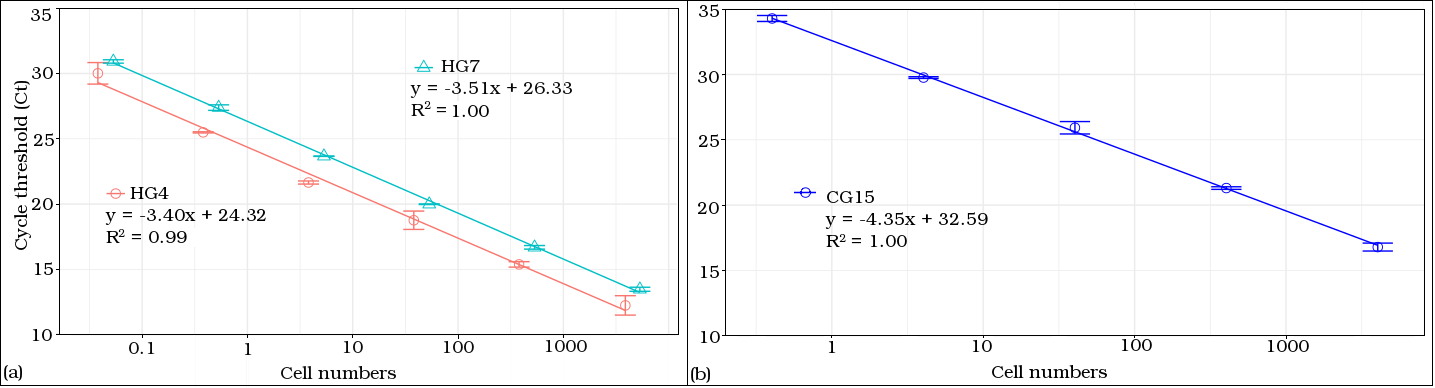
\includegraphics[scale=.22]{Fig2_cell-based-stds-merged.png}
\caption{Cell based qPCR standard curves of (a) \emph{G. lapillus} strains HG4 (circle) and HG7 (triangle); and (b) \emph{G. polynesiensis} strain CG15. Error bars represent the deviation of technical replicates during reactions.}
\label{fig:stdCurve}
\end{figure} 
\FloatBarrier
\begin{figure}
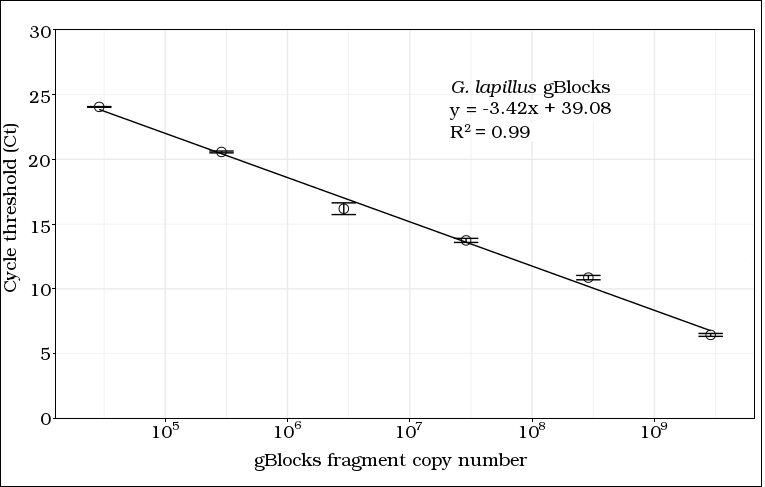
\includegraphics[scale=.4]{Fig3_gblocks-standards.png}
\caption{Gene based gBLocks qPCR standard curves of (a) \emph{G. lapillus} and (b) \emph{G. polynesiensis}. Error bars represent the deviation of technical replicates during reactions.} %Error bars represent the deviation of technical replicates during reactions.}
\label{fig:lapigblocks}
\end{figure}
\FloatBarrier
% font: URW Bookman L, size 18
%needs scale bar
\FloatBarrier 
\begin{figure} 
\includegraphics[scale=2]{Fig4_Heron-positive-negative-samplingsites.png} 
\caption{\emph{G. lapillus} presence at the sampling sites around Heron Island. The spatial replicates for each site are set up as shown in (a); the sites in (b) linked to numbering in Fig. ~\ref{fig:samplesites} where positive (green) and negative (red) as per Supplementary Table 1.} 
\label{fig:envposneg}
\end{figure} 
\FloatBarrier

\begin{figure} 
\includegraphics[scale=.8]{Fig5_Env-sample-sites-plot.png} 
\caption{Detection of \emph{G. lapillus} per spatial replicate at each sampling site, cell numbers as normalised to HG7 standard curve (Fig. ~\ref{fig:stdCurve}A). Spatial replicates coloured as per macroalgal substrate,\ where \emph{Chnoospora} sp. are green, \emph{Sargassum} sp. are blue, \emph{Padina} sp. are red and mixed macroalgal substrates are yellow (see Supplementary Table 1).} 
\label{fig:envHG7}
\end{figure} 
\FloatBarrier
 \section*{Acknowledgements}
Gratitude to Dr. Adachi and Dr. Nishimura for supplying \emph{G. scabrosus}, Michaela Larsson for supplying \emph{G. carpenteri} as well as Dr. Kirsty Smith and Dr. Lesley Rhodes for supplying \emph{G. cheloniae}, all three species were used for DNA for cross reactivity assessment. 

\section*{Conflict of interest}
The authors report no conflict of interest in conducting this study.

\section*{Author contribution}
The environmental samples from Heron Island were collected by G. Kohli. 
DNA from environmental samples was extracted by A. L. Kretzschmar, A. Verma and G. Kohli. %Reference \emph{G. polynesiensis} cultures from the Cook Islands were established from a field trip attended by Arjun Verma, G. Kohli and S. Murray. %not necesary because Arjun wasn't on lapillus paper & everyone else should be on the paper too then
The \emph{G. polynesiensis} assay was designed by A. L. Kretzschmar. 
The \emph{G. lapillus} assay was designed by A. L. Kretzschmar. The assays were tested for specificity, sensitivity, standard curves generated and environmental screening conducted by A. L. Kretzschmar. 
The manuscript was drafted by A. L. Kretzschmar and revised by all authors.

\FloatBarrier
\newpage
\bibliographystyle{apa}
%\bibliographystyle{apacite}
%\bibliographystyle{acm}
\bibliography{references.bib}
\end{document}